\section{Use Case and Quality Attribute Scenario}
\label{sec:use_case_and_qas}
This Section introduces the use case and the specified two Quality Attribute Scenarios (QAS's).
The QAS's are developed based on the use case.

\subsection{Use cases}
\label{sec:use_case}
For this project, two use cases have been chosen. One relating to one of the general Industry 4.0 QAs, and one for a QA specific to this system.

\begin{table}[ht]
    \centering
    \begin{tabular}{|l|p{50mm}|}
        \hline
        \multicolumn{2}{|c|}{\textbf{Use Case 1: Firmware Update}}\\
        \hline
        Actors &  System Administrator, Production Software.\\
        \hline
        Preconditions &  A firmware update is available.\\
        \hline
        Steps & \begin{enumerate}
                    \item Software gets notified of a new firmware version.
                    \item Software reroutes production to other components.
                    \item Software shuts down one  component.
                    \item Software installs new firmware on shutdown component.
                    \item Component notifies Software when updated and running.
                    \item Software repeats step 2-5 on all other components, one at a time.
                    \item Software resumes normal routing of production.
                    \item Software marks update as successful.
                \end{enumerate}\\
        \hline
        Postconditions & The production software is updated with the new firmware, and all affected components are notified.\\
        \hline
    \end{tabular}
    \caption{Use Case 1: Firmware Update}
    \label{tab:useCase1}
\end{table}
Use Case 1, as seen in Table \ref{tab:useCase1}, relates to the availability quality attribute, as the system should be able to continue running, even though a firmware update is scheduled. This way, machine can stay up to date, hopefully minimizing errors, while not halting production.

\begin{table}[ht]
    \centering
    \begin{tabular}{|l|p{50mm}|}
        \hline
        \multicolumn{2}{|c|}{\textbf{Use Case 2: Faulty Product Detection}}\\
        \hline
        Actors &  Quality Assurance System, Production System.\\
        \hline
        Preconditions &  The production process is ongoing.\\
        \hline
        Steps & \begin{enumerate} 
                    \item QA System continuously monitors the system.
                    \item QA System detects a faulty beer product.
                    \item QA System triggers an alert.
                    \item Fault handling detects alert, and discards bottle without disrupting production.
                \end{enumerate}\\
        \hline
        Postconditions & The faulty product is identified and discarded, without halting production.\\
        \hline
    \end{tabular}
    \caption{Use Case 2: Faulty Product}
    \label{tab:useCase2}
\end{table}
While Use Case 2, as seen in Table \ref{tab:useCase2}, is also constrained to the availability quality attribute, this part is more to demonstrate the quality attribute correctness. A requirement in this system is, that no faulty product is shipped to customers, meaning every faulty bottle will have to be discarded, before reaching the end of the production system. This means, that the software observing the bottle, must always be able to identify a faulty bottle with certainty, at each step of the production. 

The reason for choosing a non-general I4.0 QA, is that we thought it would be more interesting to work with a QA that was tailored to what we wanted to make. Since it is a I4.0 system, availability, interoperability, and deployability will have to be taken into account no matter what. We wanted to see, how we could accommodate a new requirement, that would be constrained to the required QA's of I4.0 systems, meaning that the solution to the Correctness QA, must in no way, interfere with the three other QA's. 

\subsection{Quality attribute scenarios}
\label{sec:qas}

A Quality attribute Scenario has been designed for each use case. One relating to availability during firmware update, and one relating to correctness during continuous quality assurance.

Figure \ref{fig:AQAS} shows the scenario of applying a new firmware update to certain production machines. This process is ideally fully automatic, meaning that once software developers have finished the update, and published it, the system will automatically detect a new update, schedule the update to an opportune time. Update might not be scheduled instantly, as the system could be operating at 100\% due to a large order, meaning that even though the system would not be halted during the update, throughput should still be expected to fall a bit, due to being, at least, one machine down. If the system knows that after the current order, it will be operating at 70\%, then it should schedule it there. Once a machine had been flagged for update, the system will route all production away from the flagged machine, and production will continue. Once the update is successful, the machine is flagged as ready, and is then included in the production system again. Then, another machine is flagged for update and so on. If the update fails, first step may be to try again, and if it still fails, update may end up getting rejected, and reverted to the old build, meaning developers, will have to identify and fix bugs, before machines can be updated.

\begin{figure}[h]
    \centering
    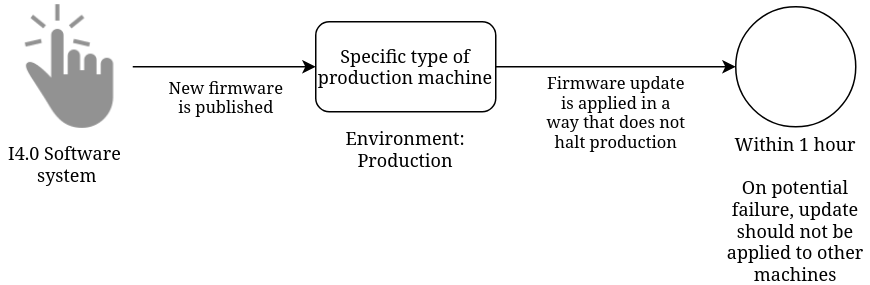
\includegraphics[width=\linewidth]{Images/Availibility.png}
    \caption{Availability Quality Attribute Scenario}
    \label{fig:AQAS}
\end{figure}

Figure \ref{fig:CQAS} show the scenario for software correctness. This scenario is only concerned with identifying faulty bottles, and not the handling of faulty bottles. By limiting it to only identifying, the scenario is more specific, and less broad, meaning a more thorough analysis of the specific attribute an be achieved. At each step of production, there will be a chance of failure. A bottle might be uncleaned or under-poured or a label may be printed crookedly. It is not a question of if that will happen, but rather a certainty that it will happen sometimes. Therefore the system needs to be able to identify faults at each step of the production. Assuming four production steps, if a fault is produced at step 1, that leaves 3 steps, that would still be processed, even though the bottle needs to be discarded anyways, which is money out the windows. Therefore, a part of the QA system will be present after each production step, where an image sensor/ computer vision will scan the bottle, and send data to an image processing service, which will then flag the bottle as either faulty or non-faulty. If a bottle is identified as faulty, the image processing service will publish an alert to a bus. This must be completed before the next production step, as to not waste resources. 

\begin{figure}[h]
    \centering
    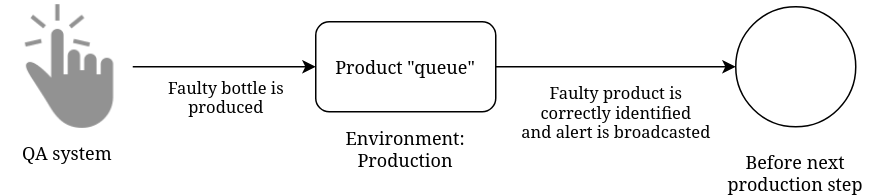
\includegraphics[width=\linewidth]{Images/Correctness.png}
    \caption{Correctness Quality Attribute Scenario}
    \label{fig:CQAS}
\end{figure}

